\documentclass[aspectratio=169]{beamer}
\usepackage[utf8]{luainputenc}
\usepackage[TS1,T1]{fontenc}
\usepackage{babel}
\usetheme[pagenum,navbar,ddc]{tud}
\usepackage{xcolor}
\usepackage{listings}
\usepackage{tikz}
\usepackage{mathtools}
\usepackage[labelformat=empty,font=scriptsize]{caption}
\usepackage{multicol}
\usepackage{marvosym}
\usepackage{wasysym}

\newcommand{\theory}[1]{\text{Th}\left( #1 \right)}
\newcommand{\lang}[1]{\text{L(}#1{)}}

\title{Decidability \protect\\\mdseries of Logical Theories\strut}
\subtitle{Proseminar Theoretical Computer Science}
\author{Lucas Waclawczyk}

\newcommand*\inmm[1]{\pgfmathsetmacro\inmmwert{#1 / 1mm}\inmmwert}
\makeatletter
\newcommand*\inpt[1]{\setlength\@tempdima{#1}\the\@tempdima}
\makeatother

\AtBeginSection[]{\partpage{\usebeamertemplate***{part page}}}
\begin{document}
	\mode<presentation>{\setbeamertemplate{tud background}[image/shaded]{Seminarraum.jpg}{0.7}}
	\maketitle
	
	\mode<presentation>{\setbeamertemplate{page number in footline}[frame][text and total]}
	\frame{\frametitle{Inhalt}\tableofcontents}
	
	\section{Basics}
	\begin{frame}{Automata}
		\begin{figure}
			\only<1>{
				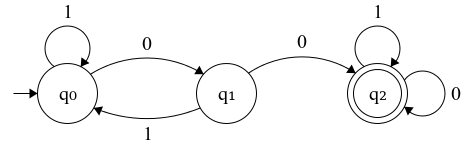
\includegraphics[width=.7\linewidth]{automata_small}
				\caption{Example automaton that accepts all binary strings containing "00"\\source: \hyperlink{ref:automata}{[1]}}
			}
			\only<2>{
				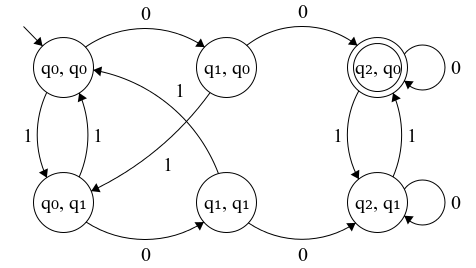
\includegraphics[width=.7\linewidth]{automata_big}
				\captionsetup{justification=centering,margin=0cm}
				\caption{Example automaton that accepts all binary strings containing an even number of "1"\\source: \hyperlink{ref:automata}{[1]}}
			}
		\end{figure}
	\end{frame}

	\begin{frame}{Turing Machines}
		\begin{figure}
			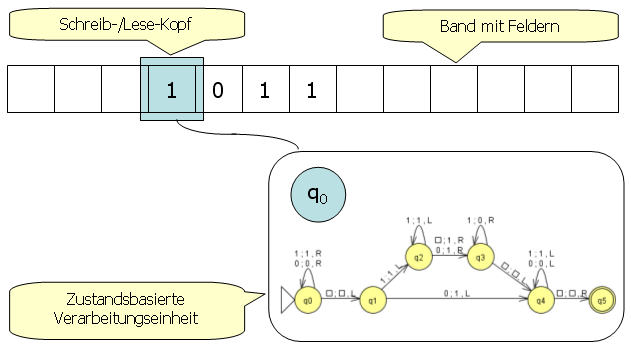
\includegraphics[width=.7\linewidth]{turing_machine}
			\caption{Example turing machine\\source: \hyperlink{ref:turing}{[2]}}
		\end{figure}
	\end{frame}

	\begin{frame}{First-Order Logic}
		\[
			\forall q \: \exists p \: \forall x, y \:\: [p>q \wedge (x, y > 1 \rightarrow xy \neq p)]
		\]
		\vspace{-.3cm}
		\only<4>{
			\[
				= \quad \forall q \: \exists p \: \forall x, y \:\: \Bigg[
					R_{1}(p, q) \wedge \Big(
						\big(
							R_{1}(x, 1) \wedge R_{1}(y, 1)
						\big) \rightarrow R_{2}(x, y, p)
					\Big)
				\Bigg]
			\]
		}
		\only<2->{\centering"There are infinitely many prime numbers."}
		
		\vspace{.25cm}
		\only<3->{\noindent\rule[.25ex]{\textwidth}{.3pt}}
		\vspace{.25cm}
		\begin{tabular}{p{.5\linewidth}p{.5\linewidth}}
			\only<3->{ 
				\begin{itemize}
					\only<3->{\item \emph{universe} $ \mathcal{U} $
						\begin{itemize}
							\item set of assignable variable values
							\item here $ \mathbb{N} $
						\end{itemize}
					}
				\only<1-4>{\end{itemize}&}
				\only<4>{\begin{itemize}}
					\only<4->{\item \emph{model} $ \mathcal{M} $
						\begin{itemize}
							\item universe with assignment of relations
							\item here $ (\mathbb{N},\: >_{2},\: (\times \neq)_{3}) $
						\end{itemize}
					\end{itemize}
					}
			}
			\only<5->{
				&
				\begin{itemize}
					\only<5->{\item \emph{language} $ \lang{\mathcal{M}} $
						\begin{itemize}
							\item sentences that make sense in $ \mathcal{M} $
							\item here $ \lang{\mathbb{N},\: >_{2},\: (\times \neq)_{3}} $
						\end{itemize}
					}
					\only<6->{\item \emph{theory} $ \theory{\mathcal{M}} $
						\begin{itemize}
							\item true sentences formed with $ \mathcal{M} $
							\item here $ \theory{\mathbb{N},\: >_{2},\: (\times \neq)_{3}} $
						\end{itemize}
					}
				\end{itemize}
			}
		\end{tabular}
	\end{frame}

	\begin{frame}{What Is Decidability?}
		\visible<1->{
			Generally:
			\begin{itemize}
				\item $ M, N $ sets, $ \varphi \in M $
				\item $ N $ decidable $ \coloneqq $ there is an algorithm that decides whether $ \varphi \in N $
			\end{itemize}
		}
		\vspace{1cm}
		\visible<2->{
			For logic:
			\begin{itemize}
				\item $ \mathcal{M} $ model, $ \varphi \in \lang{\mathcal{M}} $
				\item $ \theory{\mathcal{M}} $ decidable $ \coloneqq $ there is an algorithm that decides whether $ \varphi $ is true in $ \mathcal{M} $
			\end{itemize}
		}
	\end{frame}

	\section{$ \theory{\mathbb{N}, +} $ -- A Decidable Theory}
	\begin{frame}{Theorem 1}
		$ \theory{\mathbb{N}, +} $ is decidable
		
		\vspace{1cm}
		\uncover<2->{i.e., there is an algorithm that can decide, whether a sentence $ \varphi \in \lang{\mathbb{N}, +} $ is true or false.}
	\end{frame}

	\begin{frame}{Proof of Theorem 1}
		Let $ i \in \mathbb{N} \setminus \{0\} $ and define
		\[
			\Sigma_{i} \quad\coloneqq\quad
			\left\{
				\begin{pmatrix}
					0\\
					\vdots\\
					0\\
					0
				\end{pmatrix},
				\begin{pmatrix}
					0\\
					\vdots\\
					0\\
					1
				\end{pmatrix},
				\begin{pmatrix}
					0\\
					\vdots\\
					1\\
					0
				\end{pmatrix}, \dots,
				\begin{pmatrix}
					1\\
					\vdots\\
					1\\
					0
				\end{pmatrix},
				\begin{pmatrix}
					1\\
					\vdots\\
					1\\
					1
				\end{pmatrix}
			\right\}
			\quad \subset\quad
			\{0, 1\}^{i}
		\]
		and $ \Sigma_{0} \coloneqq \{()\} $. An example for a word in $ \Sigma_{2} $:
		\[
			\begin{pmatrix}
				0\\
				1
			\end{pmatrix}
			\begin{pmatrix}
				1\\
				0
			\end{pmatrix}
			\begin{pmatrix}
				1\\
				1
			\end{pmatrix}
			\quad \sim \quad
			\begin{pmatrix}
				3\\
				5
			\end{pmatrix}
		\]
	\end{frame}

	\begin{frame}{Proof of Theorem 1}
		\visible<1->{
			Now, let 
			\begin{itemize}
				\setlength{\itemsep}{1em}
				\item $ i \in \{1, \dots, l\} $
				\item $ \varphi = Q_{1} x_{1} \dots Q_{l} x_{l} [\psi] \in \lang{\mathbb{N}, +} $ \hspace{.3cm} where $ Q_{1}, \dots, Q_{l} \in \{\forall, \exists\} $
				\item $ \varphi_{i} \coloneqq Q_{i+1} x_{i+1} \dots Q_{l} x_{l} [\psi] $ \: and by convention $ \varphi_{l} \coloneqq \psi $
			\end{itemize}
		}
	
		\vspace{.3cm}
		\visible<2>{
			Also, for $ a_{1}, \dots, a_{i} \in \mathbb{N} $, let $ \varphi_{i}(a_{1}, \dots, a_{i}) $ be $ \varphi_{i} $ with all occurrences of $ x_{j} $ replaced by $ a_{j} $ for $ j  \in \{1, \dots, l\} $.
			
			\[
				\Longrightarrow \qquad
				\varphi_{l} \:\: \text{ is only a Boolean expression.}
			\]
		}
	\end{frame}

	\begin{frame}{Proof of Theorem 1}
		\visible<1->{
			Take
			\begin{itemize}
				\item an automaton that accepts simple addition ($ a + b = c $)
				\item an automaton that accepts boolean "and" expressions ($ p \wedge q $)
				\item an automaton that accepts boolean "or" expressions ($ p \vee q $)
				\item an automaton that accepts boolean "not" expressions ($ \neg p $) 
			\end{itemize}
		}
		\vspace{.3cm}
		\visible<2->{
			Combine them (closure, union, intersection, complementation) to get the automaton $ A_{l} $ that accepts tuples $ (a_{1}, \dots, a_{l}) \in \mathbb{N}^{l} $ for which $ \varphi_{l}(a_{1}, \dots, a_{l}) $ is true.
			
			\vspace{.3cm}
		}
		\visible<3->{
			\textbf{Important:} There is an algorithm that constructs $ A_{l} $ from $ \varphi_{l} = \psi $.
		}
	\end{frame}

	\begin{frame}{Proof of Theorem 1}
		\visible<1->{
			If $ Q_{i} = \exists $, construct automaton $ A_{i} $ from $ A_{i+1} $ by
			\begin{itemize}
				\item copying all states
				\item adding a new start state
				\item making $ A_{i} $ guess the right $ a_{i+1} $ indeterministically
			\end{itemize}
		}
	
		\vspace{.3cm}
		\visible<2->{
			If else $ Q_{i} = \forall $, use complementation twice ($ \forall x_{i} \varphi_{i+1} = \neg \exists x_{i} \neg \varphi_{i+1} $)
		}
		
		\vspace{.3cm}
		\visible<3->{
			$ \Longrightarrow \qquad A_{i} $ accepts input $ (a_{1}, \dots, a_{i}) \in \mathbb{N}^{i} \quad \Leftrightarrow \quad \varphi_{i} $ is true
		}
	
		\vspace{.3cm}
		\visible<4->{
			$ \Longrightarrow \qquad A_{0} $ accepts input $ () \quad \Leftrightarrow \quad \varphi_{0} = \varphi $ is true
		}
	
		\vspace{.3cm}
		\visible<5->{
			Let the algorithm return "$ \varphi \in \theory{\mathbb{N}, +} $" $ \quad \Leftrightarrow \quad A_{0} $ accepts input $ () $
		}
	\end{frame}

	\section{$ \theory{\mathbb{N}, +, \times} $ -- An Undecidable Theory}
	\begin{frame}{Theorem 2}
		$ \theory{\mathbb{N}, +, \times} $ is undecidable
		
		\vspace{1cm}
		\uncover<2->{i.e., there is no algorithm that can decide, whether a sentence $ \varphi \in \lang{\mathbb{N}, +} $ is true or false.}
	\end{frame}

	\begin{frame}{Proof Idea for Theorem 2}
		\begin{itemize}
			\visible<1->{
				\item The word problem for Turing machines is undecidable.
			}
			\visible<2->{
			\item There is a mapping reduction that translates
				\begin{itemize}
					\item a Turing machine $ M $ and a string $ w $
					\visible<3->{
						\item to a formula $ \varphi_{M, w} \in \theory{\mathbb{N}, +, \times} $ that contains only one free variable $ x $, such that
					}
					\visible<4->{
						\item $ \varphi_{M, w} $ is true $ \: \Leftrightarrow \: x $ is a (suitably encoded) computation history of $ M $ with which $ M $ accepts $ w $
					}
				\end{itemize}
			}
		\end{itemize}
	
		\vspace{.3cm}
		\visible<5->{
			Assume $ \theory{\mathbb{N}, +, \times} $ is decidable.
		
			$ \Longrightarrow \quad $ The formulas $ \exists x \varphi_{M, w} \in \theory{\mathbb{N}, +, \times} $ are decidable.
		}
	
		\visible<6->{
			$ \Longrightarrow \quad $ The word problem for Turing machines is decidable.
		}
	
		\visible<7->{
			$ \Longrightarrow \quad $ \Lightning
		}
	\end{frame}

	\begin{frame}{Thinking further...}
		Assumptions:
		\begin{itemize}
			\item [A$ _{1} $] Proofs can be checked by a machine.
			\item [A$ _{2} $] Provable statements are true.
		\end{itemize}
		
		\vspace{.3cm}
		\visible<2->{
			Lemmas:
			\begin{enumerate}
				\item \label{item1} The provable statements of $ \theory{\mathbb{N}, +, \times} $ are Turing recognizable.
				\\\textbf{Proof idea:} Just try all possible (suitably encoded) proofs.
				\visible<3->{
					\item There is a true statement in $ \theory{\mathbb{N}, +, \times} $ that is not provable.
					\\\textbf{Proof idea:} Contradiction to Theorem 2 by using \ref{item1}. 
				}
			\end{enumerate}
		}
	\end{frame}

	\section{Gödel's Incompleteness Theorem}
	\begin{frame}{A True, Unprovable Statement}
		We can construct a true statement in $ \theory{\mathbb{N}, +, \times} $, that is not provable.
		
		\visible<2->{
			\vspace{.3cm}
			\textbf{Construction:}
			Let $ M $ be a Turing machine that operates as follows.
			\begin{itemize}
				\item Delete the input
				\item Look for proof of $ \neg \exists x [\varphi_{M, 0}] \in \theory{\mathbb{N}, +, \times} $
				\item Accept on proof, reject if no proof can be found
			\end{itemize}
		}
		
		\vspace{.3cm}
		\visible<3->{
			$ \Longrightarrow \quad \neg \exists x [\varphi_{M, 0}] $ is the wanted statement.
		}
	\end{frame}

	\begin{frame}{Gödel's Method}
		\begin{itemize}
			\visible<1->{
				\item Construct the statement "This statement cannot be proved by the axioms."
			}
			\visible<2->{
				\item Argue against just adding this statement to the axiom.
			}
		\end{itemize}
	
		\vspace{.3cm}
		\visible<3->{
			$ \Longrightarrow \qquad $ Incompleteness \: \smiley
		}
	\end{frame}

	\section{Conclusion}
	\begin{frame}{Conclusion}
		$ \Longrightarrow \qquad $ There are (very simple) indecidable logical theories.
		
		\vspace{.3cm}
		\visible<2->{
			$ \Longrightarrow \qquad $ Mathematics cannot be mechanized.
		}
		
		\vspace{.3cm}
		\visible<3->{
			$ \Longrightarrow \qquad $ No sound logical system can be complete.
		}
	\end{frame}

	\section{References}
	\begin{frame}{References}
		\begin{itemize}
			\item [{[1]}] Martin Alessandro - Own work, CC BY-SA 4.0, \url{https://commons.wikimedia.org/w/index.php?curid=75082873} \label{ref:automata}
			\item [{[2]}] \url{https://www.inf-schule.de/grenzen/berechenbarkeit/turingmaschine/station_turingmaschine} \label{ref:turing}
			\item [{[3]}] Michael Sipser: Introduction to the Theory of Computation. Thomson Course Technology, 2006
			\item [{[4]}] \url{https://www.youtube.com/watch?v=O4ndIDcDSGc}
			\item [{[5]}] Prof. Dr. Franz Baader: Skript Theoretische Informatik und Logik (Sommersemester 2020), TU Dresden
		\end{itemize}
	\end{frame}
\end{document}
